\documentclass[10pt,a4paper]{book}
\usepackage[utf8]{inputenc}
\usepackage[T1]{fontenc}
\usepackage{amsmath}
\usepackage{amsfonts}
\usepackage{amssymb}
\usepackage{graphicx}
\usepackage{minted}
\usemintedstyle{colorful}
%\definecolor{bg}{HTML}{282828} % from https://github.com/kevinsawicki/monokai
%\setminted{bgcolor=bg,breaklines=true}
\setminted{breaklines=true}
\begin{document}
\title{Data Structures}
\author{Andrew Rosen}
\date{}
\maketitle
\tableofcontents




\chapter{Introduction}

\section{What is a Data Structures Course}
Data Structures is all about defining the different ways we can organize data.


\section{Why This Book?}

\subsection{Where Does This Book Fit Into a Computer Science Curriculum }

Education in Computer Science is based around three core topics: translating the steps of solving a problem into a language a computer can understand, organizing data for solving problems, and techniques that can be used to solve problems. % reword
These courses typically covered in a university's introductory course, data structures course, and algorithms course respectively, although different universities decide exactly what content fits in which course.
Of course, there is are lot more concepts in computer science, from operating systems and low level programming,  to networks and how computers talk to each other. However, all these concepts rely on the knowledge gained in the core courses of programming, data structures, and algorithms.

 

This textbook is all about Data Structures, the middle section between learning how to program and the more advanced problem solving concepts we learn in Computer Science. 
Here, we focus on mastering the different ways to organize data, recognize the internal and performative differences between each structure, and learn to recognize the best (if there is one) for a given situation.


\subsection{What Are My Base Assumptions about the Reader?}

This textbook assumes that the student has taken a programming course that has covered the basics.
Namely: data types such as ints, doubles, booleans, and strings; if statements, for and while loops; and object orient programming.
The first writeup of the textbook will be done in Java, but I will try to add as much Python into the book as well.


\section{To The Instructor}


\section{To The Student}


%\section{Science and Art}


\chapter{The Array}

\section{Array Operations}

\section{Finding Values in an Array}

\chapter{Analyzing Algorithms}

\subsection{Cost}
\subsubsection{Time}
\subsubsection{Space}
\subsubsection{Energy}
\subsubsection{Other costs - Bandwidth}

\section{Big O Notation}
\subsection{Space Complexity}

\section{The Formal Mathematics of Big O Notation}
\section{Other Notations}

\chapter{Lists}
The first data structure we will be studying is the list.
The list is by far the most relatable data structure, as humans deal with lists on a regular basis.

\section{What is a list?}
When you get right down to it, lists are defined by order.


\begin{minted}{Java}
public static <E> boolean isPermutation(List<E> listA, List<E> listB) {
	
	if(listA.size() != listB.size()) {
		return false;
	}
	for(int i  = 0; i < listA.size() ; i++){
		E item =  listA.get(i);
		int countA = 0;
		int countB = 0;
		
		for (E element : listA) {
			if(item.equals(element)){
				countA++;
			}
		}
		for (E element : listB) {
			if(item.equals(element)){
				countB++;
			}
		}
		if(countA != countB) {
			return false;
		}
	}
	return true;
}
\end{minted}



\section{ArrayLists}

\subsection{Generics}
\subsection{Building an ArrayList}

\subsection{More Restrictive or Permissive Generics}


\section{LinkedLists}


I will be presenting the directions to building a fully functional  singly-linked list and doubly-lined list.  
These directions will differ from the mechanics of how your programming language of choice implements them, but have the same time complexity for their operations.
My implementation is constructed with the goal of making the code easy to understand and the decisions that need to be for adding and removing reflect each other.
Finally, my code aims to minimize the number of null-pointer exceptions and their ilk a programmer would make.

The full implementations ca be found at the end of the Chapter.

\subsection{Building a Singly LinkedList}
We open up our linked list with a class declaration. 
If our language uses generics, we specify it there.
I'll be choosing not to inherit from the built-in list so we can focus solely on our own code and no external distractions.


In Java, our code looks like this.
\begin{minted}{Java}
public class LinkedList<E> { }
\end{minted}


In Python
\begin{minted}{python3}
class LinkedList(object):
	pass
\end{minted}


\subsubsection{The Node}
We want the Node class to be a private/internal class, so that the Node we write for a singly linked list and doubly linked list won't get mixed up in our coding environments.
This also applies for other data structures that will be using nodes.

\begin{minted}{Java}
public class LinkedList<E> { 
	
	private static class Node<E>{
		E item;
		Node<E> next;
		
		public Node(E item){
			this.item = item;
		}
	}
}
\end{minted}

In the Node private/internal/inner class (and only there), the \texttt{this} or \texttt{self} refers to the \textbf{node} rather than the list.





\subsubsection{Instance Variables and Constructor}


\begin{minted}{Java}
public class LinkedList<E> { 
	private int size;
	private Node<E> head;
	private Node<E> tail;
}
\end{minted}

\subsubsection{Adding}
When we add items to a linked list, 


When we do any kind of operation on a linked list, we need to think about how instance variables in a linked list will be altered. 
Fortunately, we only have three instance variables: \texttt{size}, \texttt{head}, and \texttt{tail}.
When adding to a linked list, the size will 


\subsubsection{Getting a Node at a Specific Index}

\inputminted{python3}{code/linkedlist.py}


\section{Analysis}
\chapter{Stacks}

\section{Building a Stack}

\section{Mazes - Stacks and Backtracking}



\section{Discrete Finite Automata}

\chapter{Queues}

A Queue (pronounced by saying the first letter and ignoring all the others) is a data structure which emulates the real word functionality of standing in a line (or queue, for those from Commonwealth nations).  
In a Queue, items are processed in the order they are inserted into the Queue.  So if Alice enters the Queue, followed by Bob, followed by Carla, Alice would be the first to leave the Queue, then Bob, and then Carla.

The use cases for Queues are fairly obi

\section{Linked Based Implementation} 
\section{Array Based Implementation}
We could use 


\chapter{Recursion}

\section{Recursive Mathematics}

\section{Recursive Problem Solving}

\subsection{Recursive Backtracking}
\subsection{Recursive Combinations}



\section{Recursion and Puzzles}


\section{Recursion and Art}
\section{Recursion and Nature}


\chapter{Trees}


\section{Binary Search Trees}

A diagram of a binary search tree.  It is made up of nodes, represented by circles, and edges (also called links or branches), represented by arrows.  


\section{Heaps}


\subsection{Priority Queues}

\section{Trees and Heaps in Java}
\chapter{Sorting}


\section{Quadratic-Time Algorithms}

\subsection{Bubble Sort}

\subsection{Selection Sort}

\subsection{Insertion Sort}


\section{Log-Linear Sorting Algorithms}

\subsection{Tree Sort}
\subsection{Heap Sort}
\subsection{Quick Sort}
\subsection{Merge Sort}



\section{Unique Sorting Algorithms}


\subsection{Shell Sort}

\subsection{Radix Sort}

\section{State of the Art Sorting Algorithms}

\subsection{Tim Sort}
\subsection{Quick Sort}
\subsection{Distributing and Parallelization}


\chapter{Sets and Maps}
\section{Sets}
\section{Maps}
\section{Hash Tables}
\subsection{Creating a Hash Function}
\section{Map Reduce}


\chapter{Graphs}
\section{Introduction and History}


\section{Qualities of a Graph}

\subsection{Undirected Edges}

\subsection{Directed Edges}

\subsection{Weighted Edges}

\section{Directed Acyclic Graphs}


\section{Building a Graph}

\subsection{Adjacency List}
\subsection{Adjacency Matrix}


\section{Graph Algorithms}

\subsection{Searching and Traversing}

\subsubsection{Breadth First Search}

\subsubsection{Depth First Search}


\subsection{Shortest Path}
\subsection{Topological Sorting}
\subsection{Minimum Spanning Trees}


\section{Graphs, Humans, and Networks}

\subsection{The Small World}
\subsubsection{The Milgram Experiment}
\subsubsection{The Less-Known Milgram Experiment}

\subsection{Scale Free Graphs}


\section{Graphs in Art and Nature - Voronoi Tessellation}

\begin{figure}
	\centering
	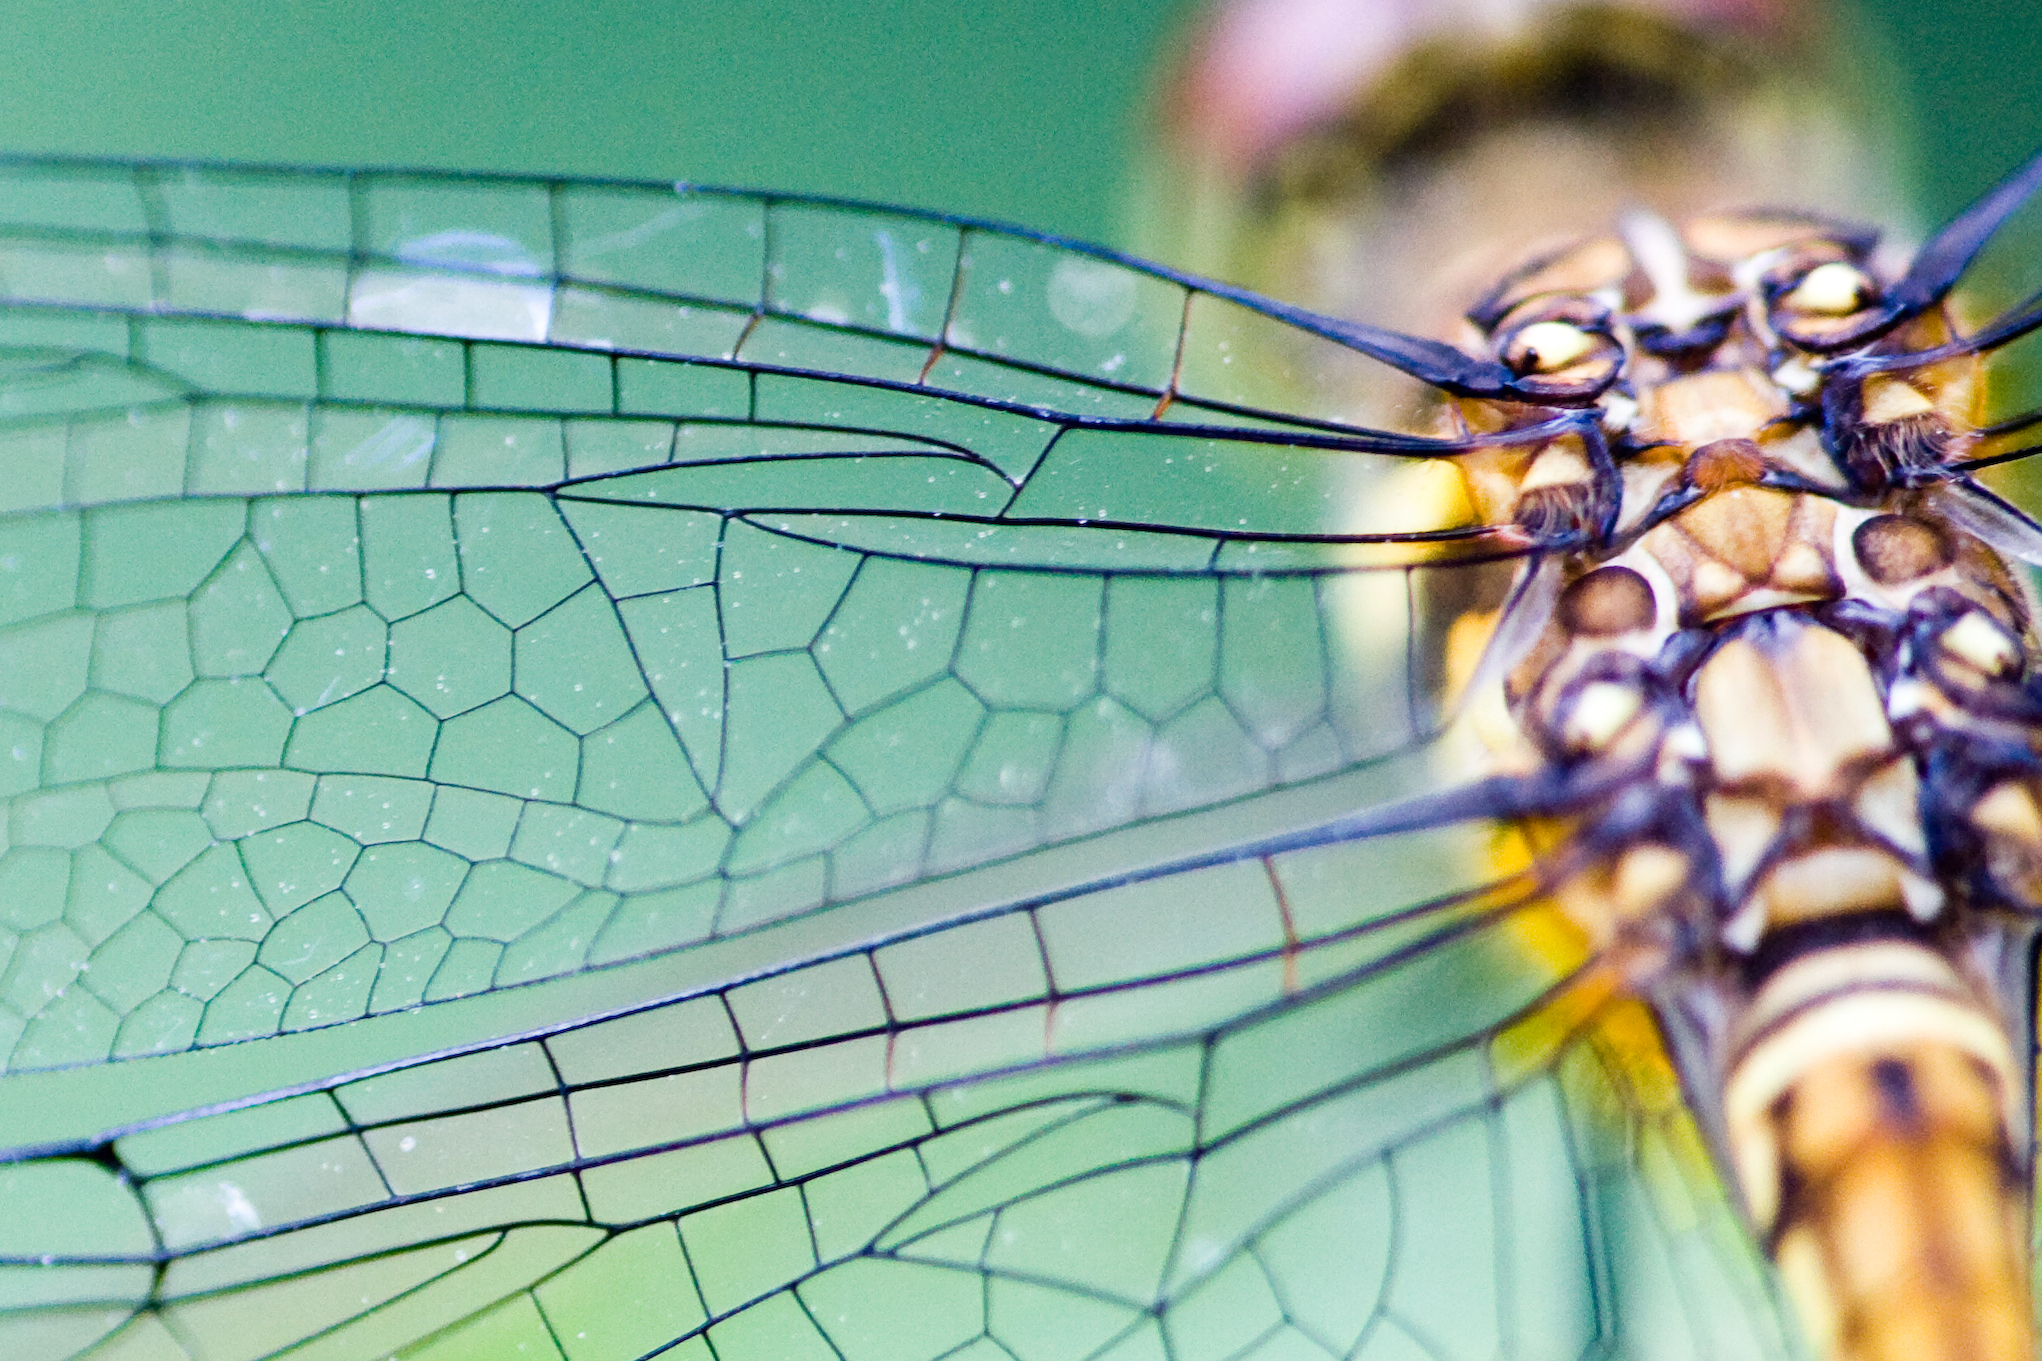
\includegraphics[width=0.7\linewidth]{pics/dragonfly_wing_joi_ito}
	\caption{The wings of a dragonfly. Credit: Joi Ito (CC BY 2.0)}
	\label{fig:dragonflywingjoiito}
\end{figure}


\section{Distributed Hash Tables}





\section{A Nontechnical Introduction to NP-Completeness}

\subsection{The Traveling Salesperson Problem (TSP)}
\subsection{The Longest Path Problem}
\subsection{The Rudrata/Hamiltonian Path Problem}
\chapter{Other Data Structures}
\section{Skip Lists}

\end{document}